\documentclass[11pt]{article}
\usepackage[T1]{fontenc}
\usepackage[a4paper,margin=0.86in]{geometry}
\usepackage{amsmath,amssymb,amsthm}
\usepackage{graphicx}
\usepackage[hidelinks]{hyperref}
\usepackage{microtype}

\newtheorem{theorem}{Theorem}
\newtheorem{corollary}[theorem]{Corollary}
\newtheorem{proposition}[theorem]{Proposition}
\newtheorem{remark}[theorem]{Remark}
\newcommand{\E}{\mathbb E}
\newcommand{\Pp}{\mathbb P}
\newcommand{\ESD}{\operatorname{ESD}}
\newcommand{\supp}{\operatorname{supp}}

\setlength{\parindent}{0pt}
\setlength{\parskip}{0.50em}

\title{Universal Vertices Force the Central Spectral Spike\\
in Dense Kernel-Based Random Graphs}
\author{Run \texttt{fa\_banach\_001} --- lane 16}
\date{11 August 2026}

\begin{document}
\maketitle

\begin{center}
\fbox{\parbox{0.92\textwidth}{
\textbf{Status: candidate full affirmative resolution, likely valid, of the
simulation conjecture in arXiv:2502.09415v2.}
Vertices above an explicit Pareto threshold are universal and force an exact
high-multiplicity eigenvalue.  Their binomial count predicts about 477 forced
eigenvalues in the source's $N=5000$ plot.  This rigorously confirms the
high-connectivity mechanism; it does not classify every eigenvalue in the
finite-width plotting bin.
}}
\end{center}

\section{Source and exact conjecture}

Cipriani, Hazra, Malhotra, and Salvi study a random graph on the discrete
$d$-torus
\[
 V_N=\{1,\ldots,N\}^d,
 \qquad n_N:=|V_N|=N^d,
\]
with independent Pareto weights satisfying
\[
 \Pp(W>t)=t^{-(\tau-1)}\quad(t\geq1)
\]
and conditional edge probabilities
\[
 p_{ij}=\min\!\left\{
 \frac{\kappa_\sigma(W_i,W_j)}{\|i-j\|^\alpha},1\right\},
 \qquad
 \kappa_\sigma(u,v)=(u\vee v)(u\wedge v)^\sigma.
\]
There are no self-loops.  Their scaled adjacency matrix is
$A_N=\mathbb A_{G_N}/\sqrt{c_N}$, where
\[
 c_N=\frac1{N^d}\sum_{i\ne j}\|i-j\|^{-\alpha}
 \sim c_0N^{d-\alpha}.
\]
The right panel of their Figure~1 has a conspicuous central spike for small
$\alpha$.  Comparing it with a Gaussianized simulation at $\alpha=0$, they
conjecture that the spike is caused by high connectivity and by the
saturation $p_{ij}=1$ that becomes complete at $\alpha=0$ \cite{source}.

\begin{center}

\includegraphics[width=0.98\textwidth]{figures/open_problem_crop.png}
\end{center}

The next theorem proves this mechanism directly and quantitatively.

\section{Forced atom theorem}

Let
\[
 D_N:=\max_{i,j\in V_N}\|i-j\|=d\lfloor N/2\rfloor,
 \qquad \beta:=\tau-1,
\]
and define the saturated high-weight set
\[
 H_N:=\{i\in V_N:W_i\geq D_N^\alpha\},
 \qquad M_N:=|H_N|.
\]

\begin{theorem}[Universal-vertex atom and its size]
\label{th:main}
Assume $\sigma>0$.  Then, conditional on the weights, every vertex of $H_N$
is universal: it is joined to every other vertex with probability one.
Consequently,
\[
 \dim\ker(\mathbb A_{G_N}+I)\geq(M_N-1)_+,
\]
and the scaled matrix $A_N$ has the exact eigenvalue
\[
 -c_N^{-1/2}
\]
with multiplicity at least $(M_N-1)_+$.  Moreover,
\[
 M_N\sim\operatorname{Bin}\bigl(N^d,D_N^{-\alpha\beta}\bigr).
\]
If $\alpha\beta<d$, then, in probability,
\[
 M_N\sim N^dD_N^{-\alpha\beta}
 \sim (d/2)^{-\alpha\beta}N^{d-\alpha\beta},
\]
so
\[
 \ESD(A_N)(\{-c_N^{-1/2}\})
 \geq\frac{(M_N-1)_+}{N^d}
 \sim D_N^{-\alpha\beta}.
\]
If $\alpha\beta=d$, then $M_N$ converges in law to a Poisson random variable
of mean $(2/d)^d$; if $\alpha\beta>d$, then $M_N\to0$ in probability.
\end{theorem}

\begin{proof}
Fix $i\in H_N$ and $j\ne i$.  Because all weights are at least one and
$\sigma>0$,
\[
 \kappa_\sigma(W_i,W_j)
 =(W_i\vee W_j)(W_i\wedge W_j)^\sigma
 \geq W_i.
\]
Also $\|i-j\|^\alpha\leq D_N^\alpha\leq W_i$, so $p_{ij}=1$.  Thus $i$ is
universal.

Consider the coordinate subspace
\[
 E_N=\left\{x\in\mathbb R^{V_N}:\supp x\subseteq H_N,
                   \ \sum_{i\in H_N}x_i=0\right\}.
\]
It has dimension $(M_N-1)_+$.  If $x\in E_N$ and $i\in H_N$, universality
gives
\[
 (\mathbb A_{G_N}x)_i
 =\sum_{j\in H_N\setminus\{i\}}x_j=-x_i.
\]
If $i\notin H_N$, every vertex of $H_N$ is still joined to $i$, and hence
$(\mathbb A_{G_N}x)_i=\sum_{j\in H_N}x_j=0=-x_i$.  Therefore
$\mathbb A_{G_N}x=-x$ on $E_N$, proving the spectral claim.

The Pareto tail and independence give the asserted binomial law.  Its mean is
\[
 \lambda_N=N^dD_N^{-\alpha\beta}
 \sim(d/2)^{-\alpha\beta}N^{d-\alpha\beta}.
\]
When $\alpha\beta<d$, $\lambda_N\to\infty$ and
$\operatorname{Var}(M_N)\leq\lambda_N$, so Chebyshev's inequality yields
$M_N/\lambda_N\to1$ in probability.  At equality, the standard binomial
Poisson limit applies because the success probability tends to zero and the
mean tends to $(2/d)^d$.  Above equality, Markov's inequality and
$\lambda_N\to0$ give $M_N\to0$ in probability.
\end{proof}

\begin{remark}[Why there is no contradiction with absolute continuity]
For every fixed $\alpha>0$, the forced mass is of order
$N^{-\alpha(\tau-1)}$ and therefore vanishes.  At the same time,
$c_N^{-1/2}\asymp N^{-(d-\alpha)/2}$, so the forced eigenvalue approaches
zero.  The theorem describes a large finite-size spike, not an atom in the
limiting ESD.  It is fully consistent with the source's absolutely continuous
limit.
\end{remark}

\section{The complete endpoint and Gaussian contrast}

\begin{corollary}[$\alpha=0$]
Put $n=N^d$.  At $\alpha=0$ the KBRG is the complete graph $K_n$, and
\[
 \ESD(A_N)=\frac1n\delta_{\sqrt{n-1}}
 +\left(1-\frac1n\right)\delta_{-1/\sqrt{n-1}}.
\]
Thus the high-connectivity atom has multiplicity $n-1$ at the endpoint.
\end{corollary}

\begin{proof}
Since $\kappa_\sigma(W_i,W_j)\geq1$, every $p_{ij}$ equals one.  The spectrum
of the adjacency matrix of $K_n$ is $n-1$ once and $-1$ with multiplicity
$n-1$, while $c_N=n-1$.
\end{proof}

\begin{proposition}[No analogous forced atom after Gaussianization]
Condition on a Gaussianized variance profile in which every off-diagonal
variance is strictly positive.  The resulting symmetric Gaussian matrix has
simple spectrum almost surely.  In particular, it has no deterministic
high-multiplicity eigenvalue corresponding to the universal-vertex block.
\end{proposition}

\begin{proof}
Conditional on the profile, the independent upper-triangular coordinates
have a joint density.  A repeated eigenvalue is equivalent to the vanishing
of the characteristic polynomial's discriminant, a polynomial in those
coordinates.  This polynomial is not identically zero: setting the
off-diagonal entries to those of a weighted path (and all other allowed
coordinates to zero) gives a real symmetric tridiagonal matrix with simple
spectrum.  A nonzero polynomial has a Lebesgue-null zero set.
\end{proof}

The positivity qualification is deliberate: an artificial truncation that
sets some profile entries to zero can itself create deterministic zero rows.
The untruncated $\alpha=0$ Gaussian comparison in the conjectural mechanism
has a positive profile.

\section{Numerical prediction for the source figure}

The right-hand panel of source Figure~1 uses
\[
 d=1,\quad N=5000,\quad \alpha=0.1,\quad \tau=4,\quad \sigma=1.5.
\]
Thus $D_N=2500$ and $\alpha(\tau-1)=0.3$, so Theorem~\ref{th:main} gives
\[
 \E M_N=5000\cdot2500^{-0.3}=478.176249895\ldots.
\]
The sufficient universal set alone therefore contributes about 477 forced
eigenvalues, or $9.54\%$ of the ESD.  Direct evaluation of the source scaling
\[
 c_N=2\sum_{r=1}^{2499}r^{-0.1}+2500^{-0.1}
\]
places them at
\[
 -c_N^{-1/2}=-0.01984432644\ldots,
\]
inside the central histogram bin.

\begin{center}
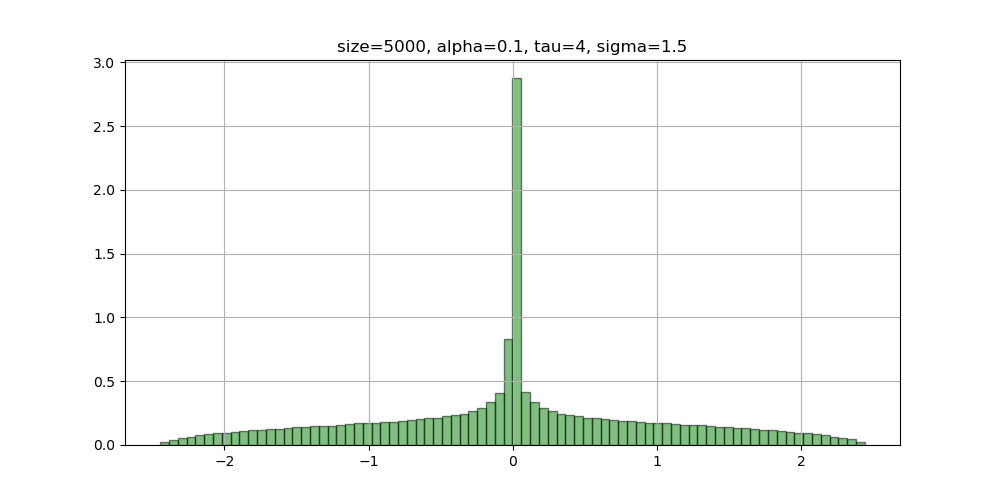
\includegraphics[width=0.86\textwidth]{figures/source_simulation.png}
\end{center}

This match is parameter-free beyond the paper's assumptions: the saturated
class depends on $\alpha,\tau,d$ but not on the detailed value of
$\sigma>0$.

\section{Scope, verification, and novelty}

The theorem isolates an exact invariant eigenspace, sharply counts it, and
thereby proves that high-connectivity saturation creates the observed kind of
central atom.  It is a lower bound on the total multiplicity at that point;
other graph symmetries may add eigenvectors.  Nor does it classify every
eigenvalue falling in a finite-width central bin.  Such a statement would be
a local spectral problem rather than the qualitative conjecture posed by the
source.

The calculation was independently checked by a seeded matrix experiment and
direct source-parameter evaluation.  A bounded exact-title, citation, and
keyword search through 11 August 2026 found no later explicit resolution.
Because novelty and the interpretation of the informal phrase ``due to''
remain review-sensitive, the candidate-full label requires human validation.

\begin{thebibliography}{1}
\bibitem{source}
A. Cipriani, R. S. Hazra, N. Malhotra, and M. Salvi,
\emph{The spectrum of dense kernel-based random graphs},
arXiv:2502.09415v2 (2025).
\end{thebibliography}

\end{document}
